\subsection{Išskirčių tyrimas}
\paragraph{} Tyrėme HDI ir vaisinugmo rodiklio išskirtis, norėdami vėliau vykdyti sąryšių analizę, nes kai kurie duomenys gali iškraipyti kai kuriuos skaičiavimus(pavyzdžiui, Pirsono(angl. Pearson) koreliacijos koeficiento). 
Išskirtis tyrėme pasitelkdami kvartilių metodą. Tai reiškia, kad reikšmę laikėme sąlygine išskirtimi, jei ji priklausė intervalui $[Q1-3IQR; Q1-1,5IQR) \cup (Q3+1,5IQR; Q3+3IQR]$. O išskirtimi laikėme tokią reikšmę, kuri priklauso intervalui $(-\infty; Q1-3IQR] \cup [Q3+3IQR; \infty)$. \\\par
Šių kintamųjų išskirtis ir pasiskirstymą iliustruoja stačiakampės diagramos:

\begin{multicols}{2}
    \begin{figure}[H]
        \centering
        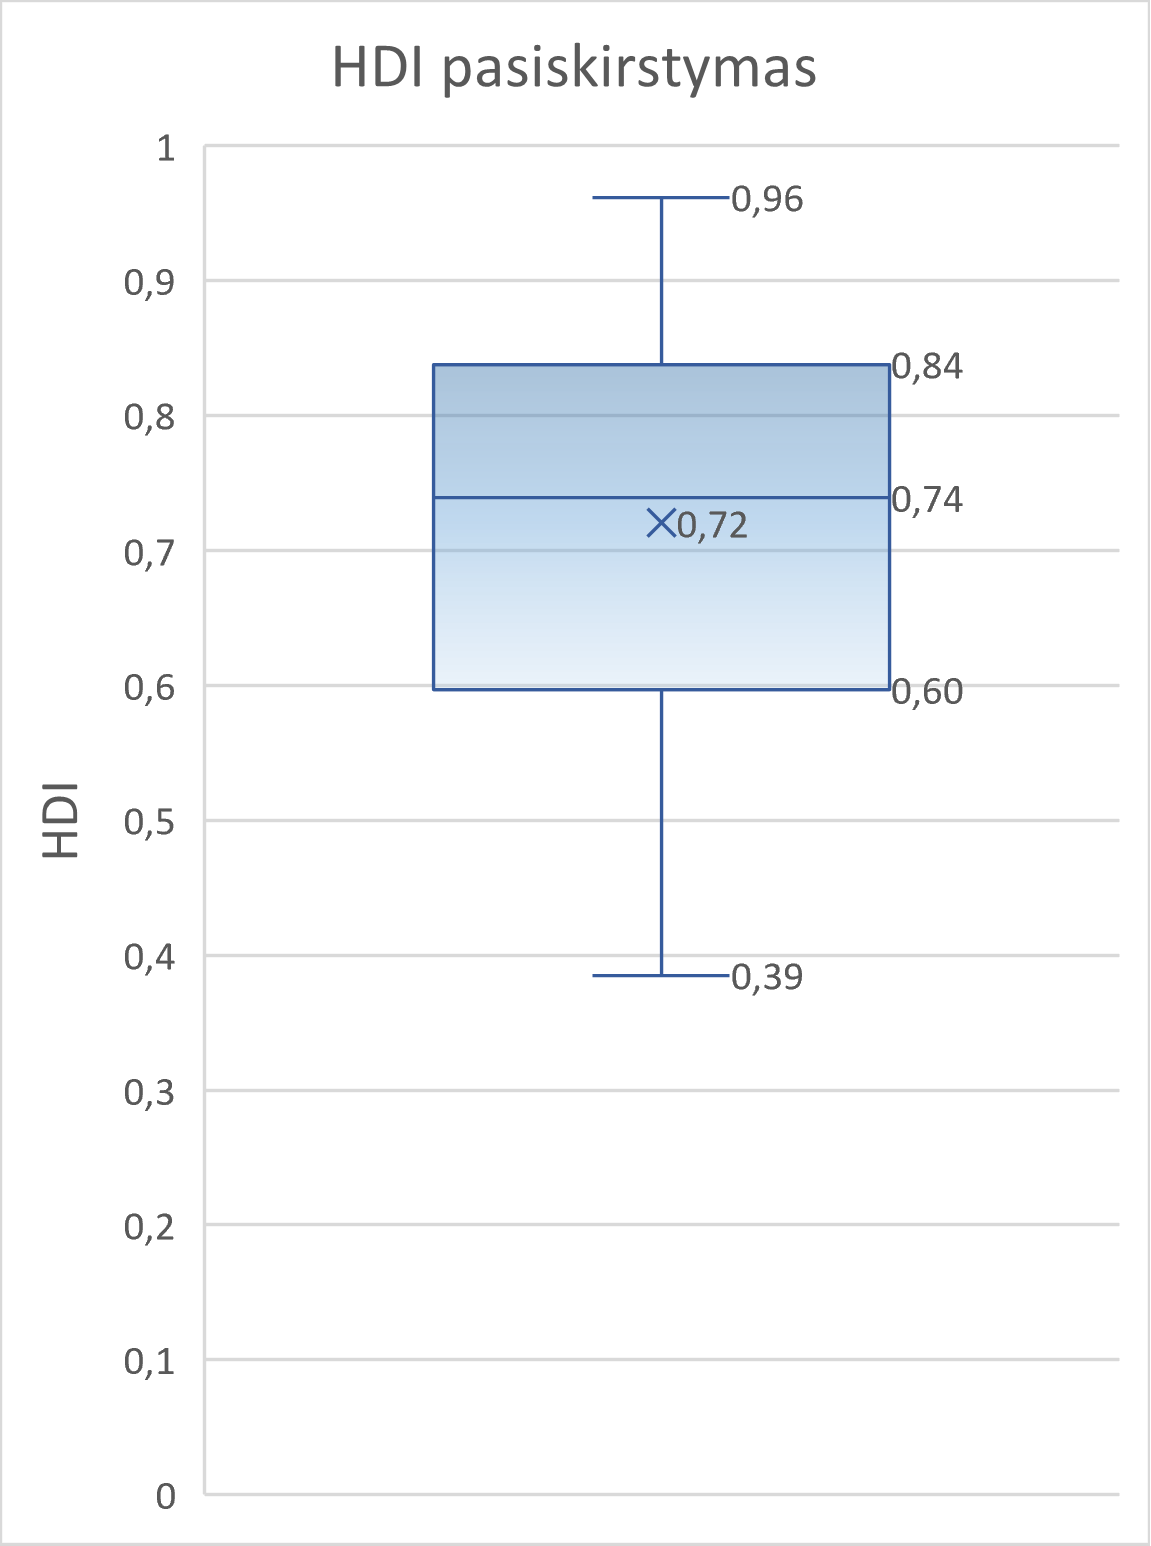
\includegraphics[width=.3\textwidth]{pic/box.png}
        \caption{HDI stačiakampė diagrama}
    \end{figure}
    \begin{figure}[H]
        \centering
        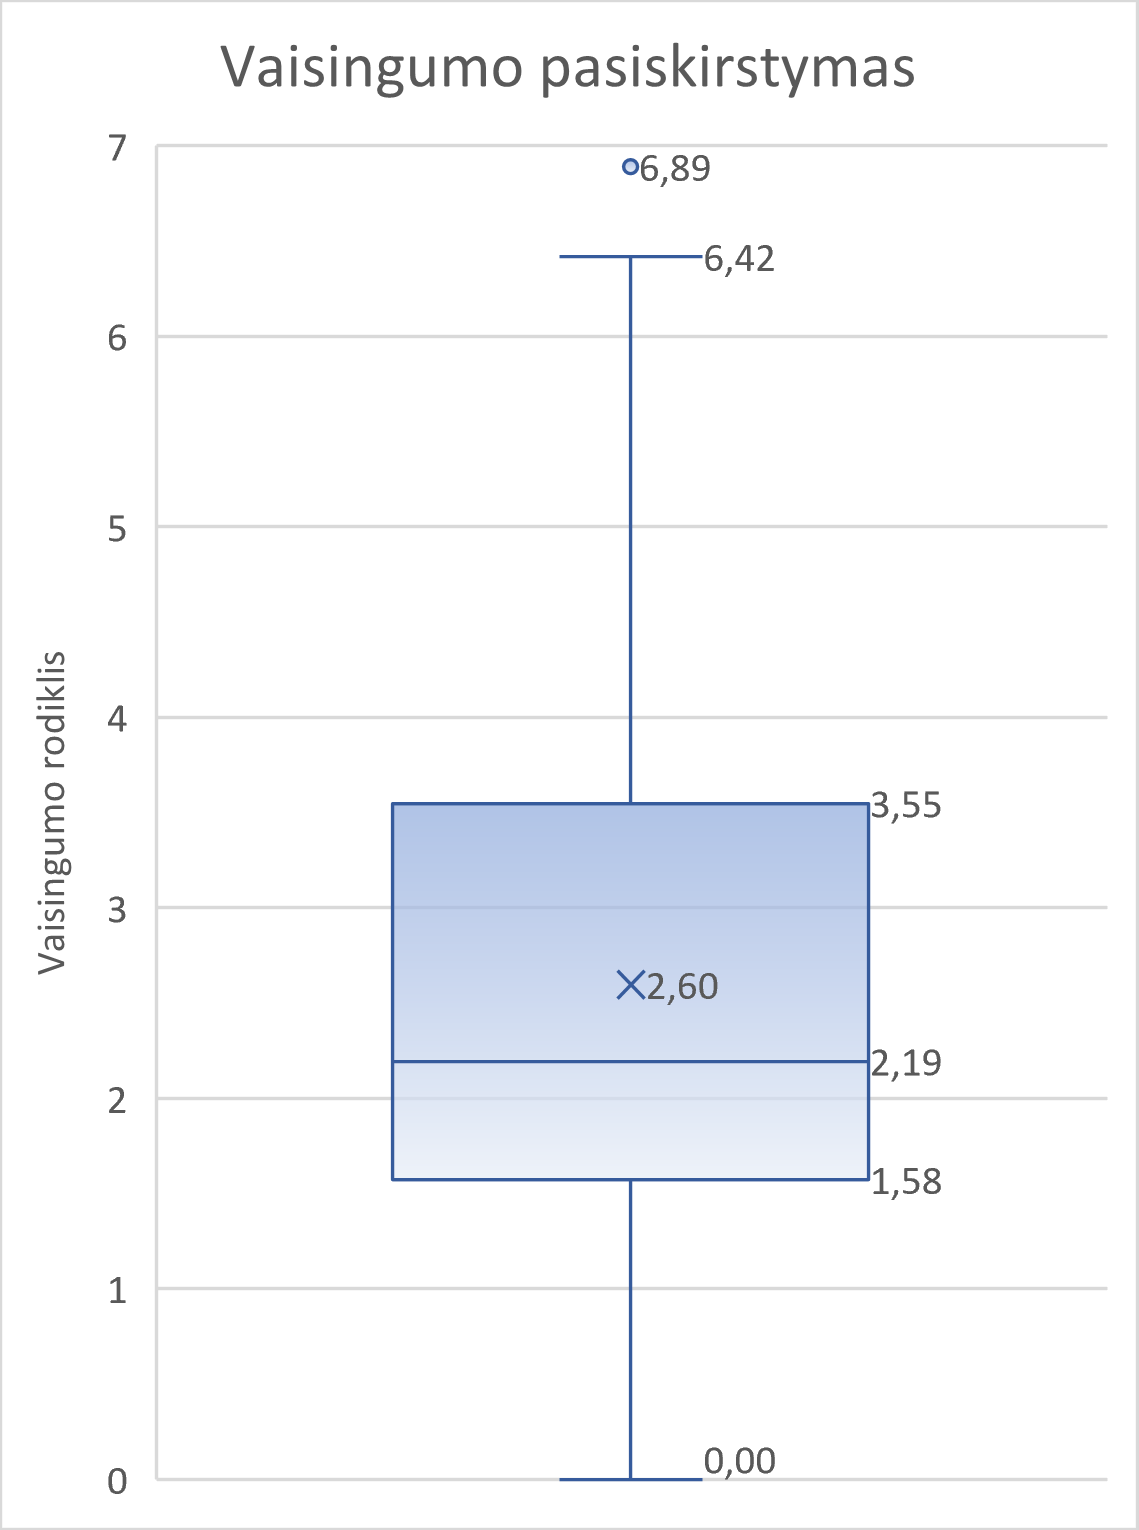
\includegraphics[width=.3\textwidth]{pic/box2.png}
        \caption{Vaisingumo rodiklio stačiakampė diagrama}
    \end{figure}
\end{multicols}
\pagebreak

\subsection{Koreliacijos tyrimas}
Pamatavome vaisingumo ir HDI bei vaisingumo ir aukštojo išsilavinimo procento rodiklių koreliacijas. Tai padarėme, pritaikydami Pirsono(angl. Pearson) koreliacijos koeficientą. Jis paskaičiuojamas pagal formulę: 
\begin{equation}
r = \frac{\sum\limits_i (x_i - \bar{x})(y_i - \bar{y})}{\sqrt{\sum\limits_i(x_i - \bar{x})^2}\sqrt{\sum\limits_i(y_i - \bar{y})^2}}
\end{equation}

Tyrimo rezultatus pateikiame lentelėje:
\begin{table}[H]
\begin{center}
    \begin{tabular}{|c|c|}
        \hline
        \textbf{Lyginti kintamieji} & \textbf{Pirsono koreliacijos koeficientas} \\\hline
        HDI ir Vaisinigumo rodiklis & -0,819 \\\hline
        Aukštojo išsilavinimo procentas ir vaisingumo rodiklis & -0,399 \\\hline
    \end{tabular}
    \caption{Koreliacijos skaičiavimų rezultatai}
\end{center}
\end{table}

Šių kintamų sąryšius iliustruoja sklaidos diagramos:
\begin{multicols}{2}
\diagrama{pic/vias_hdi_rod.png}{Gyventojų vaisingumo rodiklio ir HDI sklaidos diagrama}
\diagrama{pic/gyv_vais_kor.png}{Gyventojų vaisingumo rodiklio ir aukštojo išsilavinimo procento sklaidos diagrama}
\end{multicols}

\pagebreak

\subsection{Aukštąjį išsilavinimą gavusiųjų suaugiusiųjų pasiskirtsymo tyrimas} 

Aukštąjį išsilavinimą gavusių suaugiusiųjų pasiskirtsymą iliustruoja histograma:
\diagrama{pic/histo.png}{Aukštąjį išsilavinimą gavusių procentas.}

\subsection{Vaisingumo pasiskirstymas pasaulyje}
Tirdami šį pasiskirstymą pagal šalis nubrėžiame žemėlapį:
\diagrama{pic/map.png}{Vaisingumo rodiklis įvairiose pasaulio šalyse.}

Tirdami šį pasiskirstymą pagal žemynus nubrėžiame skritulinę diagramą:
\diagrama{pic/pie_2020.png}{Skritulinė diagrama, vaizduojanti vaisingumą įvairiuose žemynuose}

\subsection{Vaisingumo rodiklis Baltijos šalyse}
Mums buvo svarbu nustatyti, kaip skiriasi minėti rodikliai tarp Baltijos šalių.
Tam mums pravertė stulpelinė diagrama:
\diagrama{pic/balt.png}{Įvairūs rodikliai Baltijos šalyse}

Taip pat, mes tyrėme, kaip keitėsi Baltijos šalių vaisingumo rodiklis tarp 1960 ir 2021 metų.
\diagrama{pic/vais_balt.png}{Baltijos šalių vaisingumo rodiklis įvairiais metais}
